\documentclass[tikz,border=4pt]{standalone}
\usetikzlibrary{positioning}

\begin{document}
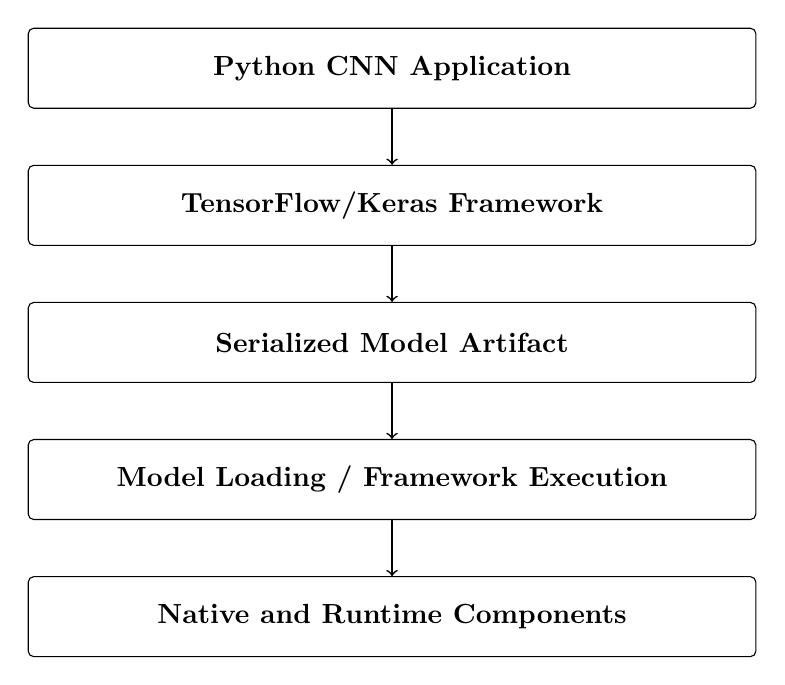
\begin{tikzpicture}[
  stage/.style={
    draw,
    rounded corners=2pt,
    text width=3.5in,
    minimum height=0.4in,
    align=center,
    font=\bfseries,
    inner sep=5pt
  },
  node distance=0.28in
]
\node[stage] (application) {Python CNN Application};
\node[stage, below=of application] (framework) {TensorFlow/Keras Framework};
\node[stage, below=of framework] (artifact) {Serialized Model Artifact};
\node[stage, below=of artifact] (loading) {Model Loading / Framework Execution};
\node[stage, below=of loading] (native) {Native and Runtime Components};

\draw[->, semithick] (application) -- (framework);
\draw[->, semithick] (framework) -- (artifact);
\draw[->, semithick] (artifact) -- (loading);
\draw[->, semithick] (loading) -- (native);
\end{tikzpicture}
\end{document}
